% ============================================================
\chapter{SymPy III: integrais e aplicações}
\label{cap:aula9}
% ============================================================

\begin{objetivos}
\begin{itemize}
  \item calcular integrais indefinidas, definidas e impróprias com \py{sp.integrate};
  \item reconhecer quando não há primitiva elementar e calcular o valor numérico da integral;
  \item calcular áreas entre curvas e volumes de sólidos de revolução;
  \item visualizar somas de Riemann e obter a integral como limite dessas somas;
  \item calcular integrais duplas em retângulos e em regiões mais gerais.
\end{itemize}
\end{objetivos}

\begin{roteiro}
0--20 min & Integrais indefinidas e definidas; verificação por derivação; o objeto \py{sp.Integral}.\\
20--30 min & Integrais impróprias; integrais sem primitiva elementar e valores numéricos.\\
30--45 min & Somas de Riemann (gráfico e limite).\\
45--65 min & Área entre curvas; volume de sólidos de revolução.\\
65--75 min & Integrais duplas.\\
75--90 min & Exercícios.\\
\end{roteiro}

\begin{entrada}
import sympy as sp
import numpy as np
import matplotlib.pyplot as plt
x, y = sp.symbols('x y')
\end{entrada}

% ------------------------------------------------------------
\section{Integrais indefinidas e definidas}
% ------------------------------------------------------------

\begin{sintaxe}
sp.integrate(f, x)               # primitiva (sem a constante C)
sp.integrate(f, (x, a, b))       # integral definida de a até b
sp.Integral(f, (x, a, b))        # integral "por extenso" (não calcula); .doit() calcula
\end{sintaxe}

\begin{entrada}
sp.integrate(x**2, x), sp.integrate(x*sp.exp(x), x), sp.integrate(sp.exp(x)*sp.cos(x), x)
\end{entrada}
\begin{saidamat}
$\displaystyle \left( \frac{x^{3}}{3}, \  \left(x - 1\right) e^{x}, \  \frac{e^{x} \sin{\left(x \right)}}{2} + \frac{e^{x} \cos{\left(x \right)}}{2}\right)$
\end{saidamat}

\begin{atencao}
O SymPy \textbf{não escreve a constante de integração}: a resposta é uma primitiva; a família de todas as
primitivas é $F(x)+C$.
\end{atencao}

\begin{entrada}
sp.integrate(1/(x**2 - 1), x), sp.integrate(sp.sin(x)**3, x), sp.integrate(1/sp.sqrt(1 - x**2), x)
\end{entrada}
\begin{saidamat}
$\displaystyle \left( \frac{\log{\left(x - 1 \right)}}{2} - \frac{\log{\left(x + 1 \right)}}{2}, \  \frac{\cos^{3}{\left(x \right)}}{3} - \cos{\left(x \right)}, \  \operatorname{asin}{\left(x \right)}\right)$
\end{saidamat}

\begin{observacao}
O SymPy escreve $\log$ para o logaritmo natural $\ln$. Também omite o módulo: $\int\frac{dx}{x}$ aparece como
$\log(x)$, e não $\ln|x|$.
\end{observacao}

\paragraph{Conferindo por derivação.} Uma forma de verificar uma primitiva é derivá-la:

\begin{entrada}
f = x**2 * sp.sin(x)
F = sp.integrate(f, x)
print(F)
sp.simplify(sp.diff(F, x) - f)
\end{entrada}
\begin{saida}
-x**2*cos(x) + 2*x*sin(x) + 2*cos(x)
\end{saida}
\begin{saidamat}
$\displaystyle 0$
\end{saidamat}

\paragraph{Integrais definidas.} Pelo Teorema Fundamental do Cálculo, $\int_a^b f(x)\,dx=F(b)-F(a)$. O SymPy faz
isso diretamente:

\begin{entrada}
sp.integrate(x**3 + x, (x, 0, 1)), sp.integrate(sp.sin(x), (x, 0, sp.pi)), sp.integrate(sp.log(x), (x, 1, sp.E))
\end{entrada}
\begin{saidamat}
$\displaystyle \left( \frac{3}{4}, \  2, \  1\right)$
\end{saidamat}

\begin{entrada}
I = sp.Integral(x * sp.sqrt(1 + x**2), (x, 0, 2))
sp.Eq(I, I.doit())
\end{entrada}
\begin{saidamat}
$\displaystyle \int\limits_{0}^{2} x \sqrt{x^{2} + 1}\, dx = - \frac{1}{3} + \frac{5 \sqrt{5}}{3}$
\end{saidamat}

\paragraph{Cuidado com descontinuidades.} O tutorial do R. Miranda propõe ``enganar'' o SymPy com
$\int_0^3\frac{dx}{x-2}$, cujo integrando tem uma assíntota vertical em $x=2$, dentro do intervalo. Aplicar a
fórmula $F(3)-F(0)=\ln|1|-\ln|-2|$ sem pensar daria $-\ln 2$, o que está \textbf{errado}: a integral imprópria
diverge.

\begin{entrada}
sp.integrate(1/(x - 2), (x, 0, 3))
\end{entrada}
\begin{saidamat}
$\displaystyle \text{NaN}$
\end{saidamat}

\begin{maxima}
\texttt{integrate(f, x)} e \texttt{integrate(f, x, a, b)} do Maxima correspondem a \py{sp.integrate(f, x)} e
\py{sp.integrate(f, (x, a, b))} (repare nos parênteses em volta de \py{(x, a, b)}). O Maxima às vezes pergunta
``Is x positive, negative or zero?''; no SymPy declaramos as hipóteses nos símbolos
(\py{sp.symbols('a', positive=True)}).
\end{maxima}

% ------------------------------------------------------------
\section{Integrais impróprias e valores numéricos}
% ------------------------------------------------------------

O infinito é \py{sp.oo}. Integrais impróprias divergentes resultam em \py{oo}.

\begin{entrada}
sp.integrate(sp.exp(-x**2), (x, -sp.oo, sp.oo)), sp.integrate(1/x**6, (x, 1, sp.oo)), sp.integrate(1/x, (x, 1, sp.oo))
\end{entrada}
\begin{saidamat}
$\displaystyle \left( \sqrt{\pi}, \  \frac{1}{5}, \  \infty\right)$
\end{saidamat}

\begin{entrada}
p = sp.symbols('p', positive=True)
sp.integrate(1/x**p, (x, 1, sp.oo))
\end{entrada}
\begin{saidamat}
$\displaystyle \begin{cases} \frac{1}{p - 1} & \text{for}\: p > 1 \\\int\limits_{1}^{\infty} x^{- p}\, dx & \text{otherwise} \end{cases}$
\end{saidamat}

O SymPy responde ``por casos'': a integral vale $\frac{1}{p-1}$ se $p>1$ (e diverge caso contrário).

\paragraph{Funções sem primitiva elementar.} Algumas funções simples, como $e^{-x^2}$ e $\frac{\sin x}{x}$, não têm
primitiva que se escreva com funções elementares. O SymPy responde com funções especiais (a função erro
$\operatorname{erf}$, o seno integral $\operatorname{Si}$) ou devolve a integral sem calcular. Em todos os casos, o
valor numérico de uma integral definida pode ser obtido com \py{evalf}:

\begin{entrada}
sp.integrate(sp.exp(-x**2), x), sp.integrate(sp.sin(x)/x, x)
\end{entrada}
\begin{saidamat}
$\displaystyle \left( \frac{\sqrt{\pi} \operatorname{erf}{\left(x \right)}}{2}, \  \operatorname{Si}{\left(x \right)}\right)$
\end{saidamat}

\begin{entrada}
J = sp.Integral(sp.sqrt(1 + x**4), (x, 0, 1))
print(J.doit())
print(J.evalf(15))
\end{entrada}
\begin{saida}
gamma(1/4)*hyper((-1/2, 1/4), (5/4,), -1)/(4*gamma(5/4))
1.08942941322482
\end{saida}

Para $\int_0^1\sqrt{1+x^4}\,dx$ o SymPy encontrou uma resposta em termos das funções gama ($\Gamma$) e
hipergeométrica, pouco úteis na prática; o valor numérico, por outro lado, é imediato.

% ------------------------------------------------------------
\section{Somas de Riemann}
% ------------------------------------------------------------

Dividindo $[a,b]$ em $n$ partes de largura $\Delta x=\frac{b-a}{n}$ e escolhendo um ponto $x_i^*$ em cada parte, a
soma de Riemann $\sum_{i=1}^n f(x_i^*)\,\Delta x$ aproxima $\int_a^b f$. O código abaixo, adaptado do tutorial do
R. Miranda (que por sua vez se baseia no \emph{Mathematical Python}, de P. Walls), desenha as somas pela esquerda,
pelo ponto médio e pela direita.

% figura: aula09-riemann
\begin{entrada}
def f(t):
    return t**2

a, b, N = 0, 2, 8
dx = (b - a) / N
xs = np.linspace(a, b, 200)
esq = np.linspace(a, b - dx, N)          # extremos esquerdos
pontos = {"esquerda": esq, "ponto médio": esq + dx/2, "direita": esq + dx}

fig, ax = plt.subplots(1, 3, figsize=(12, 3.6), sharey=True)
for eixo, (nome, xi) in zip(ax, pontos.items()):
    eixo.plot(xs, f(xs), "b", lw=2)
    eixo.bar(esq, f(xi), width=dx, align="edge", alpha=0.35, edgecolor="b")
    eixo.plot(xi, f(xi), "r.", ms=9)
    soma = np.sum(f(xi) * dx)
    eixo.set_title(f"{nome}: soma = {soma:.4f}")
plt.show()
print("valor exato:", sp.integrate(x**2, (x, 0, 2)))
\end{entrada}
\saidafig[1.0]{aula09-riemann}
\begin{saida}
valor exato: 8/3
\end{saida}

Aumentando $N$, as três somas se aproximam de $\frac83\approx2{,}6667$. O SymPy permite fazer a conta com $n$
genérico e calcular o limite, exatamente como na definição da integral:

\begin{entrada}
n, i = sp.symbols('n i', integer=True, positive=True)
dx = sp.Rational(2) / n
Sn = sp.summation(((i*dx)**2) * dx, (i, 1, n))       # soma pela direita
print(sp.factor(Sn))
sp.limit(Sn, n, sp.oo)
\end{entrada}
\begin{saida}
4*(n + 1)*(2*n + 1)/(3*n**2)
\end{saida}
\begin{saidamat}
$\displaystyle \frac{8}{3}$
\end{saidamat}

% ------------------------------------------------------------
\section{Área entre curvas}
% ------------------------------------------------------------

A área da região entre os gráficos de $f$ e $g$, para $x\in[a,b]$, é $\int_a^b |f(x)-g(x)|\,dx$. Os limites de
integração costumam ser os pontos de interseção, obtidos com \py{solve}. Exemplo: a região entre $y=x^2$ e $y=x+2$.

\begin{entrada}
f = x + 2
g = x**2
pts = sp.solve(sp.Eq(f, g), x)
print("interseções em x =", pts)
area = sp.integrate(f - g, (x, pts[0], pts[1]))
area
\end{entrada}
\begin{saida}
interseções em x = [-1, 2]
\end{saida}
\begin{saidamat}
$\displaystyle \frac{9}{2}$
\end{saidamat}

% figura: aula09-area
\begin{entrada}
xs = np.linspace(-1.5, 2.5, 300)
F, G = sp.lambdify(x, f), sp.lambdify(x, g)
plt.plot(xs, F(xs), label="$y=x+2$")
plt.plot(xs, G(xs), label="$y=x^2$")
xr = np.linspace(-1, 2, 200)
plt.fill_between(xr, G(xr), F(xr), alpha=0.3, label="área = 9/2")
plt.legend()
plt.grid(True)
plt.show()
\end{entrada}
\saidafig[0.5]{aula09-area}

\begin{atencao}
Se as curvas se cruzam dentro do intervalo, $\int_a^b (f-g)$ \emph{não} é a área: as partes em que $g>f$ entram
com sinal negativo. Divida o intervalo nos pontos de interseção ou integre \py{sp.Abs(f - g)}.
\end{atencao}

\begin{entrada}
# área entre sen(x) e cos(x) em [0, pi]: as curvas se cruzam em pi/4
errado = sp.integrate(sp.sin(x) - sp.cos(x), (x, 0, sp.pi))
certo = sp.integrate(sp.cos(x) - sp.sin(x), (x, 0, sp.pi/4)) + sp.integrate(sp.sin(x) - sp.cos(x), (x, sp.pi/4, sp.pi))
errado, certo
\end{entrada}
\begin{saidamat}
$\displaystyle \left( 2, \  2 \sqrt{2}\right)$
\end{saidamat}

% ------------------------------------------------------------
\section{Volumes de sólidos de revolução}
% ------------------------------------------------------------

Girando em torno do eixo $x$ a região sob o gráfico de $f\ge0$, $x\in[a,b]$, obtém-se um sólido cujas seções
transversais são discos de raio $f(x)$. Seu volume é
\[
V=\pi\int_a^b f(x)^2\,dx \qquad\text{(método dos discos).}
\]

\begin{figure}[ht]
\centering
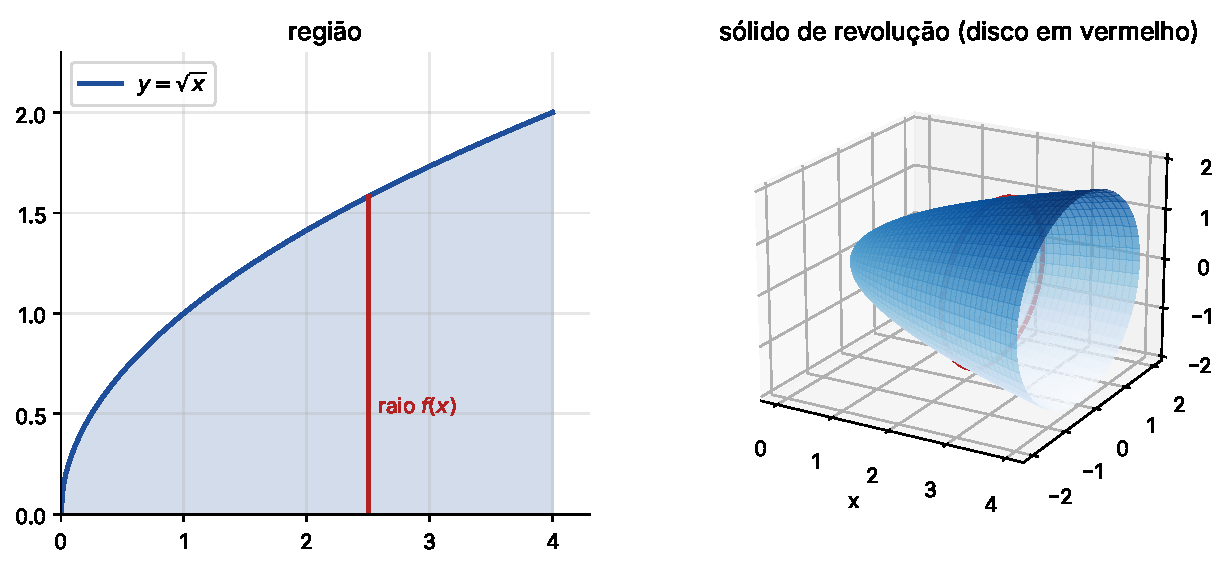
\includegraphics[width=0.8\linewidth]{aula09-revolucao}
\caption{Região sob $y=\sqrt{x}$, $0\le x\le4$, e o sólido obtido ao girá-la em torno do eixo $x$ (um paraboloide).}
\end{figure}

\begin{entrada}
V = sp.pi * sp.integrate(sp.sqrt(x)**2, (x, 0, 4))
V
\end{entrada}
\begin{saidamat}
$\displaystyle 8 \pi$
\end{saidamat}

Com um raio simbólico, deduzimos o volume da esfera girando o semicírculo $y=\sqrt{r^2-x^2}$:

\begin{entrada}
r = sp.symbols('r', positive=True)
sp.pi * sp.integrate(sp.sqrt(r**2 - x**2)**2, (x, -r, r))
\end{entrada}
\begin{saidamat}
$\displaystyle \frac{4 \pi r^{3}}{3}$
\end{saidamat}

\paragraph{Comprimento de arco.} O comprimento do gráfico de $f$ entre $a$ e $b$ é
$\int_a^b\sqrt{1+f'(x)^2}\,dx$. Para $y=\frac23x^{3/2}$, $0\le x\le3$:

\begin{entrada}
f = sp.Rational(2, 3) * x**sp.Rational(3, 2)
sp.integrate(sp.sqrt(1 + sp.diff(f, x)**2), (x, 0, 3))
\end{entrada}
\begin{saidamat}
$\displaystyle \frac{14}{3}$
\end{saidamat}

% ------------------------------------------------------------
\section{Integrais duplas}
% ------------------------------------------------------------

Integrais iteradas são feitas indicando várias variáveis, \textbf{da mais interna para a mais externa}:
\py{sp.integrate(f, (y, c, d), (x, a, b))} calcula $\int_a^b\!\left(\int_c^d f\,dy\right)dx$.

\begin{entrada}
sp.integrate(x*y**2, (y, 0, 2), (x, 0, 3))         # retângulo [0,3] x [0,2]
\end{entrada}
\begin{saidamat}
$\displaystyle 12$
\end{saidamat}

Em uma região do tipo $\{(x,y): a\le x\le b,\ g_1(x)\le y\le g_2(x)\}$, os limites da integral interna dependem
de $x$. Por exemplo, a região entre $y=x^2$ e $y=x$:

\begin{entrada}
sp.integrate(x + y, (y, x**2, x), (x, 0, 1))
\end{entrada}
\begin{saidamat}
$\displaystyle \frac{3}{20}$
\end{saidamat}

A área de uma região é a integral dupla de 1. Em coordenadas polares, $dA=r\,dr\,d\theta$: a área do círculo de raio
$R$ é

\begin{entrada}
rho, theta, R = sp.symbols('rho theta R', positive=True)
sp.integrate(rho, (rho, 0, R), (theta, 0, 2*sp.pi))
\end{entrada}
\begin{saidamat}
$\displaystyle \pi R^{2}$
\end{saidamat}

\begin{professor}
A comparação ``errado \emph{versus} certo'' na área entre seno e cosseno costuma gerar uma boa discussão. Se a
turma ainda não viu integrais duplas, a última seção pode ser omitida ou apenas mostrada. Uma atividade
alternativa é retomar a regra dos trapézios da Aula 4 e compará-la com o valor exato do SymPy.
\end{professor}

% ------------------------------------------------------------
\section{Exercícios}
% ------------------------------------------------------------

\begin{exercicio}[primitivas]{ex:9-primitivas}
Calcule e confira derivando: (a) $\int x^2e^{-x}\,dx$; (b) $\int\frac{x+3}{x^2+x-2}\,dx$; (c) $\int\sec^2 x\,dx$;
(d) $\int x\ln x\,dx$; (e) $\int\frac{dx}{1+4x^2}$.
\end{exercicio}

\begin{exercicio}[definidas e impróprias]{ex:9-definidas}
Calcule: (a) $\int_0^{\pi/2}\sin^2x\,dx$; (b) $\int_1^e\frac{\ln x}{x}\,dx$; (c) $\int_0^\infty xe^{-x}\,dx$;
(d) $\int_0^1\frac{dx}{\sqrt x}$; (e) $\int_0^1 \frac{dx}{x}$.
\end{exercicio}

\begin{exercicio}[área]{ex:9-area}
Calcule a área da região limitada por $y=x^3-x$ e $y=3x$ e faça um gráfico da região.
\end{exercicio}

\begin{exercicio}[Riemann]{ex:9-riemann}
Para $f(x)=\sqrt{x}$ em $[0,4]$, calcule numericamente as somas pela esquerda, direita e ponto médio para
$N=10, 100, 1000$ e compare com o valor exato $\frac{16}{3}$. Qual converge mais rápido?
\end{exercicio}

\begin{exercicio}[volume]{ex:9-volume}
Calcule o volume do sólido obtido girando em torno do eixo $x$ a região sob $y=e^{-x}$, $x\ge0$. Calcule também
o volume do cone obtido girando $y=\frac{R}{h}x$, $0\le x\le h$, e confira que é $\frac13\pi R^2h$.
\end{exercicio}

\begin{exercicio}[extra: valor médio e integral dupla]{ex:9-extra}
(a) O valor médio de $f$ em $[a,b]$ é $\frac{1}{b-a}\int_a^bf$. Calcule o valor médio de $\sin x$ em $[0,\pi]$.
(b) Calcule $\iint_D xy\,dA$, em que $D$ é o triângulo de vértices $(0,0)$, $(1,0)$ e $(1,1)$.
\end{exercicio}
